\documentclass[a4paper,11pt]{article}
\usepackage[utf8]{inputenc}
\usepackage[T1]{fontenc}
\usepackage[french]{babel}
\usepackage[right=2.5cm, left=2.5cm, bottom=4cm, top=3cm]{geometry}
\usepackage[ddmmyyyy]{datetime}
\usepackage[table]{xcolor}
\usepackage{lmodern,mathptmx,changepage,titlesec,hyperref,listings,lstautogobble,graphicx,array,longtable,multirow,lipsum,tikz,shorttoc,enumitem,float}
\usetikzlibrary{arrows,automata}
\usetikzlibrary{positioning}

\renewcommand{\rmdefault}{\sfdefault} %Utilisation de la police sans-serif ("Computer Modern Sans") pour la police roman
\renewcommand{\ttdefault}{pcr} 	%Utilisation d'une police "CourrierNew" pour la police monospaced (pour faire un listing manuel)
\linespread{1.15}				%Interligne

%Utilisation de liens colorés en bleu et soulignés
\hypersetup{colorlinks=true, urlcolor=blue, urlbordercolor=blue, linkcolor=black, linkbordercolor=white}
\makeatletter \Hy@AtBeginDocument{\def\@pdfborder{0 0 1} \def\@pdfborderstyle{/S/U/W 1}}\makeatother

\titlespacing*{\section} {0cm}{7ex plus 1ex minus .2ex}{1.5ex plus .2ex}
\titlespacing*{\subsection} {0cm}{4.5ex plus 1ex minus .2ex}{1.5ex plus .2ex}
\titleformat*{\section}{\LARGE\bfseries}
\titleformat*{\subsection}{\large\bfseries}
\titleformat*{\subsubsection}{\normalsize\bfseries}

\definecolor{darkgreen}{rgb}{0,0.8,0}
\definecolor{mygray}{rgb}{0.93,0.93,0.93}
\definecolor{mymauve}{rgb}{0.58,0,0.82}
\lstset{	
	language=Python,
	basicstyle=\small\ttfamily,
	backgroundcolor=\color{mygray},
	breaklines=true,
	breakatwhitespace=true,
	tabsize=3,
	frame=none,
	rulecolor=\color{black},
	keywordstyle=\color{blue}\bfseries,
	stringstyle=\color{orange},
	showstringspaces=false,
	commentstyle=\footnotesize\color{darkgreen},
	keepspaces=true,
	extendedchars=true,
	numbers=left,
	numberstyle=\tiny\color{lightgray},
	stepnumber=1,
	escapeinside={(@}{@)},
	autogobble=true,
	literate=
		{á}{{\'a}}1 {é}{{\'e}}1 {í}{{}}1 {ó}{{\'o}}1 {ú}{{\'u}}1
		{Á}{{\'A}}1 {É}{{\'E}}1 {Í}{{\'I}}1 {Ó}{{\'O}}1 {Ú}{{\'U}}1
		{à}{{\`a}}1 {è}{{\`e}}1 {ì}{{\`i}}1 {ò}{{\`o}}1 {ù}{{\`u}}1
		{À}{{\`A}}1 {È}{{\'E}}1 {Ì}{{\`I}}1 {Ò}{{\`O}}1 {Ù}{{\`U}}1
		{ä}{{\"a}}1 {ë}{{\"e}}1 {ï}{{\"i}}1 {ö}{{\"o}}1 {ü}{{\"u}}1
		{Ä}{{\"A}}1 {Ë}{{\"E}}1 {Ï}{{\"I}}1 {Ö}{{\"O}}1 {Ü}{{\"U}}1
		{â}{{\^a}}1 {ê}{{\^e}}1 {î}{{\^i}}1 {ô}{{\^o}}1 {û}{{\^u}}1
		{Â}{{\^A}}1 {Ê}{{\^E}}1 {Î}{{\^I}}1 {Ô}{{\^O}}1 {Û}{{\^U}}1
		{œ}{{\oe}}1 {Œ}{{\OE}}1 {æ}{{\ae}}1 {Æ}{{\AE}}1 {ß}{{\ss}}1
		{ç}{{\c c}}1 {Ç}{{\c C}}1 {ø}{{\o}}1 {å}{{\r a}}1 {Å}{{\r A}}1
		{€}{{e}}1 {£}{{\pounds}}1 {«}{{\guillemotleft}}1
		{»}{{\guillemotright}}1 {ñ}{{\~n}}1 {Ñ}{{\~N}}1 {¿}{{?`}}1
}

%Redéfinition de la taille de \Huge pour le titre du document
\makeatletter\renewcommand\Huge{\@setfontsize\Huge{37pt}{40}}\makeatother
\date{\today}


\title{\vspace{\fill}\textbf{\Huge Rapport}}
\author{Jean-Didier Pailleux - Maxence Joulin - Damien Thenot - Romain Robert - Robin Feron 
	\vspace{2em}\\
	\textit{Test de primalité}\\
	\textcolor{red}{https://github.com/CHPS-M1-PRIME-NUMBERS/Prime\_numbers}
	\vspace{2em}
}

\begin{document}
\pagenumbering{gobble}\clearpage
\maketitle\vspace{13em}
\begin{center}
\includegraphics[scale=0.7]{logo.png}\end{center}
\begin{flushright}\textit{Projet de Programmation numérique}\end{flushright}
\newpage
\tableofcontents
\newpage\clearpage\pagenumbering{arabic}

	\section{Introduction}
% pour l'intro si tu modifies des trucs, garde la meme mise en page malek.
	\paragraph{}Ce document est le compte-rendu de notre travail qui s'inscrit dans le cadre du module \textit{Projet de Programmation numérique} du master \textit{Calcul Haute Performance Simulation} de l'\textit{\textbf{UVSQ}}. Le sujet de ce projet a été proposé par l'encadrant Sébastien Gougeaud.
	
	\paragraph{}Ce projet découle d'un thème qui est le test de primalité, et consiste à tester si un nombre est bien premier ou non. Un nombre premier est un entier qui admet uniquement deux diviseurs distincts et positifs (1 et lui même). 
	Les nombres premiers prennent une place importante dans le domaine des mathématiques et ont des propriétés très utiles particulièrement dans le domaine de la cryptographie. La recherche de très grands nombres premiers est devenu de plus en plus captivé par beaucoup, de nombreux tests de primalité ont pu émerger, voir évoluer, devenir plus performants, et de plus en plus rapides.
	
	\paragraph{}Il existe actuellement deux types de tests de primalités, les déterministes qui permettent d'établir avec certitude le résultat et les tests probabilistes qui émettent un résultat non fiable avec une certaine probabilité d'erreur mais sont plus rapide que les tests déterministes.
	
	\paragraph{}L'objectif de ce projet consiste à implémenter plusieurs de ces tests (déterministes) et ainsi comparer leur vitesse  d'exécution. Ceci pour l'exécution des tests de primalités pour un nombre premier, et pour une exécution sur les tests avec n nombres premiers. De plus un test probabiliste sera programmé pour ainsi comparer la fiabilité du résultat et le temps que nécessite de faire cet algorithme.\\ 
	Une partie bonus nous a été proposé lors de notre entretient avec Monsieur Gougeaud qui consiste à implémenter une fonctionnalité pour déterminer si un nombre est hautement composé (c'est à dire que le nombre de ses diviseurs est supérieur strictement à tout les nombres inférieur à lui). 
	
	\paragraph{}Dans la première partie de ce document, on présentera l'architecture de notre projet (la décomposition), illustrée par un organigramme qui a été préalablement établi.\\
	Après cela, on mentionnera les différents outils et langages utilisé au cours de la phase l'implémentation.\\
	Puis dans une autre partie l'analyse des résultats établis lors des tests du projet accompagné d'un comparatif de la performance des tests.\\
	Finalement, dans les deux dernières parties, on établira un bilan quant à l'organisation interne au sein du groupe et un bilan technique du projet qui mettra en avant les limites de chaque test de primalité.
	
		
	\section{Architecture du projet}
		\subsection{Organigramme}
		L'organigramme suivant fait part de la décomposition que va adopter le projet. Le projet se décompose en trois catégories de tests pour les nombres hautement composé, les tests de primalité déterministe et les tests de primalité probabiliste. \\ 
		\begin{center}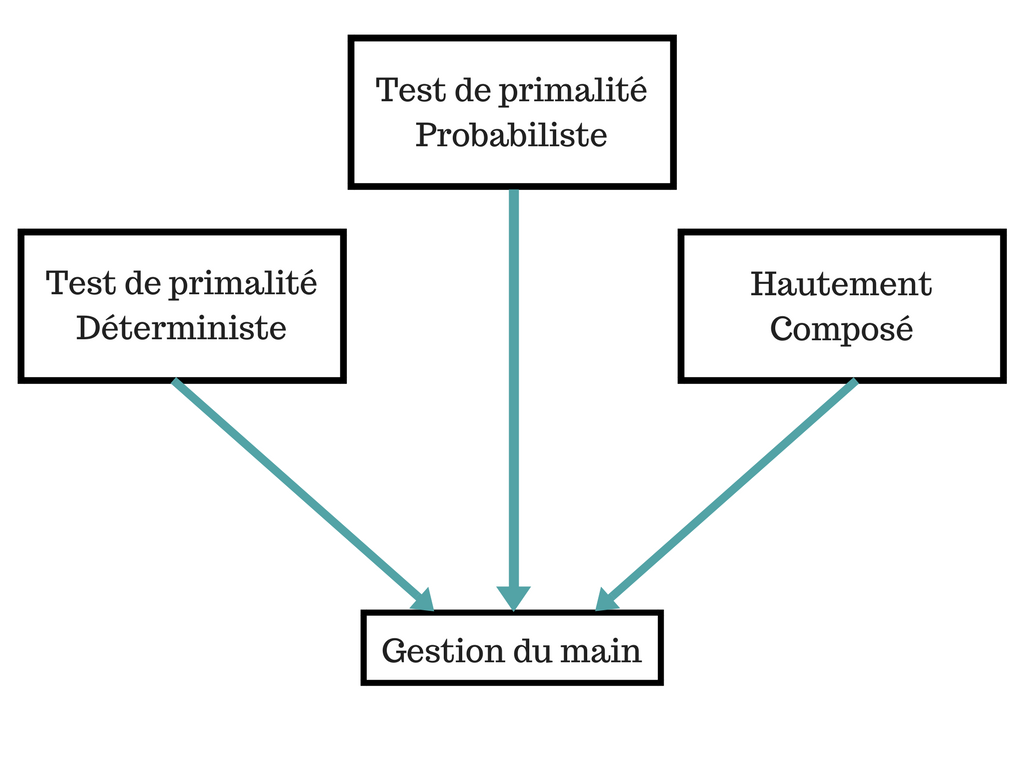
\includegraphics[scale=0.5]{organigramme.png}\end{center}
		
		\subsection{Tests de primalité}
		Au cours de ce projet il nous a été demandé d'implémenter plusieurs algorithmes pour déterminer si un nombre est premier ou non. Voici les différents tests utilisés pour ce travail:
		\begin{itemize}
			\item Méthode naïve le \textbf{crible d’Ératosthène}\footnote{zanotti.univ-tln.fr/ALGO/I51/Crible.html} utilisé pour le memory bound. Cet l'algorithme va procéder à une élimination dans une table d'entiers de 2 à N de tous les multiples de chaque entier présent dans ce tableau. En supprimant tous les multiples à la fin seuls les entiers qui ne sont multiples d'aucun autre resteront, et par conséquent ces nombres seront donc premiers. Le memory bound va donc être une liste des entiers restant à la fin de l'application du crible.\\
			
			\item Méthode naïve \textbf{l'algorithme d'Euclide} (Déterministe).\\ Les premiers algorithmes naïfs sont très simple mais couteux en temps de calcul. Un nombre est en effet premier si aucun nombre qui lui est inferieur le divise. Cet algorithme va donc essayer de diviser le nombre n dont on souhaite tester la primalité par tout ces nombres. Si l'un d'entre eux donne pour reste de la division 0, alors n n'est pas premier. Afin de limiter le nombre de calculs nécéssaires on peut se limiter à tester uniquement tout les nombres inferieurs à $\sqrt{n}$. En effet si un nombre a > $\sqrt{n}$ divise n, alors a x b = n où b est forcement plus petit que $\sqrt{n}$. Donc n aura été prouvé non premier par b avant d'essayer a.\\
On peut également utliser l'algorithme d'Euclide qui permet de trouver de manière iterative le plus grand diviseur commun de deux nombres (PGCD). Or on dit que a et b sont premiers entre eux lorsque leur PGCD est égal à 1. Il suffit donc de prouver que chaque nombre inferieur à $\sqrt{n}$ a pour PGCD 1 avec n pour dire que n est premier.
\\
Ces deux méthodes sont très simples à implementer mais deviennent très rapidement coûteuses en temps de calcul pour des nombres très grands, s'approchant de $2^{64}$ par exemple.\\
			
			\item \textbf{Pocklington} (Déterministe): Le test de primalité de Pocklington-Lehmer utilise le théorème de Pocklington pour vérifier la primalité d’un nombre.
L’algorithme consiste à utiliser une factorisation partielle du nombre N-1, où N est le nombre dont on souhaite tester la primalité. Cette factorisation partielle nous permet d’obtenir un nombre que l’on nommera A et qui doit remplir certaines conditions pour qu’on puisse appliquer le théorème.
Nous avons déjà la factorisation de A qui nous servira pour la suite de l'exécution de l’algorithme. 
La suite consiste à tester les conditions requises sur tous les facteurs premiers de A, ces conditions sont de trouver un nombre "$a$" qui mis à la puissance N-1 modulo N donne 1 et que le plus grand diviseur commun entre {\Large$\frac{a^{(N-1)}}{p}$} et N soit égal à 1, avec p le facteur premier de A tester en ce moment. Si on a trouvé un "$a$" remplissant les conditions pour chaque “p” alors on peut dire que le nombre N est premier.\\

			\item \textbf{AKS} 2002 (Déterministe) :			
			L'algorithme AKS est l’acronyme de ses créateurs (Agrawal-Kayal-Saxena). AKS est un algorithme déterministe, inconditionnel (il fonctionne peut importe l'entrée) et polynomiale c'est l'un des rares algorithmes à vérifier toutes ces propriétés. Cet Algorithme se base sur une généralisation du petit théorème de Fermat\footnote{https://fr.wikipedia.org/wiki/Test\_de\_primalit\%C3\%A9\_AKS} qui est : "Pour tout entier $n \geq 2$ et tout entier $a$ premier avec $n$, $n$ est un nombre premier si et seulement si : $(X + a)^n \equiv X^n + a$ $mod$ $n$".\\

En ce qui concerne l’algorithme il est effectuée en 5 étapes\footnote{https://en.wikipedia.org/wiki/AKS\_primality\_test}:\\
\begin{enumerate}
	\item On vérifie que $n \ne a^b$ avec $A \in N$ et $b>1$.
	\item On détermine le plus petit entier $r$ tel que l’ordre de n dans Z/rZ soit supérieur à $\log2(n)^2$.
	\item Pour tous les "$a$" compris entre 2 et le minimum entre $r$ et $n-1$ on vérifie que "$a$" ne divise pas n.
	\item Si n $\leq$ r alors n est premier.
	\item Pour $a$ allant de $1$ à ($\sqrt{\phi (r)*\log 2(n)}$) en valeur entière inférieur on vérifie que $(X + a)^n \equiv X^n + a$ (mod $X^r$ -1,n).
\end{enumerate}

Si tout ces tests sont passées on peut dire que n est premier.\\
Pour la version réalisée (2002), la complexité est de l'ordre de $\log(n)^{12}$ cependant il existe beaucoup de variante qui améliore l'algorithme (exemple en 2005 une nouvelle variante d'AKS s’exécute en $\log(n)^6$ ce qui représente une belle optimisation comparé à la version initiale). La plupart des optimisations concerne l'étape 5, elle occupe une grande partie de l'exécution de l'algorithme (On essaie de réduire le plus possible la taille de $r$ pour permettre de faire le moins d'itération possible ).\\
			
			\item \textbf{Miller-Rabin} (Probabiliste): Miller-Rabin, basé sur le petit théorème de Fermat \\ $a^p-1 \equiv 1 \pmod p$, consiste à tirer parti d'une équation ou d'un système d'équations qui sont vraies pour des valeurs premières, et à regarder si elles sont toujours vraies ou non pour un nombre dont nous voulons tester la primalité. La fonction Miller-Rabin prend en paramètre un entier n dont on souhaite vérifier la primalité et un entier k qui représente le nombre d’itération du test de Miller-Rabin plus k est élevé est plus l’analyse est précise (moins de chance d’erreurs).\\
		\end{itemize}
		
		\subsection{Nombres Hautement composés}
		Deux fonctions ont été implémenté pour les nombres hautement composés. La première fonction : 				\begin{lstlisting}
			bool highly_composite_naive(unsigned int number)
		\end{lstlisting}
		C'est une méthode naïve qui consiste à calculer le nombre de diviseur d'un nombre n et de comparer ce nombre avec le nombre de diviseurs pour tout entier k compris entre $1$ et $n-1$.
		\paragraph{}La seconde fonction est :
		\begin{lstlisting}
			bool highly_composite_def(unsigned int number)
		\end{lstlisting}
		Elle utilise la propriété sur la forme qu'un nombre hautement composé doit avoir. Un nombre hautement composé possèdent des facteurs premiers les plus petits possible. Si l'on doit prendre en considération que la décomposition d'un entier $n > 1$ en produit de facteurs premiers comme suit  $n = p_1^{c_1} * p_2^{c_2} * ... * p_k^{c_k}$ où $p_1 = 2 < p_2 = 3 < … < p_k$ sont les $k$ plus petits nombres premiers, avec $c_k$ le dernier exposant non nul.
		\paragraph{}En conséquence, pour que n soit hautement composé, il faut que $c_1 \ge c_2 \ge ... \ge c_k$. En cas de non respect de cette règle si nous échangeons deux exposants on diminue le nombre n tout en conservant exactement le même nombre de diviseurs. Un exemple pour illustrer : 18 = $2^1 * 3^2$ peut être remplacé par $12 = 2^2 * 3^1$, ces deux nombres ont tout les deux 6 diviseurs. De plus il a été montré que le dernier exposant $c_k = 1$, sauf dans deux cas particuliers $n = 4$ et $n = 36$.

	\section{Outils et langages de programmation}
		\subsection{Langages de programmation}
		Lors de la réalisation du projet, des contraintes nous ont été imposées par notre encadrant. Tout d'abord, le langage de programmation utilisé est le langage C++. Langage adapté pour la programmation procédurale et pour la programmation orientée objet. De plus, il dispose de nombreuses bibliothèques permettant de manipuler des grands entiers supérieur à $2^{64}$, de chronométrer l'exécution d'une portion du programme, et autre.\\
		Le deuxième langage est le Shell. Celui-ci faisant partie du système d'exploitation UNIX, va nous permettre d'établir un script \textit{test.sh} avec l’enchaînement de plusieurs lignes de commandes pour l'exécution de tests.
		
		\subsection{Outils}
		Pour ainsi produire le projet certains outils ont été utilisé pour obtenir le résultat présenté. En premier lieu nous avons installé la bibliothèque \textit{GMP}. Cette dernière est une bibliothèque nécessaire pour utiliser NTL, de plus il pourrait nous être utile dans le cas où l'on voudrait générer de très grands nombre car les types de base proposé par le C++ nous limite à l'utilisation de nombre de 64 bits maximum.
		\paragraph{}Ensuite le second outils utilisé est la bibliothèque \textit{NTL}, propose certaines fonctionnalité pour le calcul du PolyModulo\footnote{https://en.wikipedia.org/wiki/AKS\_primality\_test} qui nous est indispensable pour l'implémentation du test de primalité AKS. N'ayant aucune connaissance nécessaire dans le domaine mathématique sur le polymodulo, l'utilisation de cette bibliothèque nous permet d'obtenir des fonctions pour ces calculs et de façon optimisée.  
		\paragraph{}Nous avons également utilisé un service d’hébergement de gestion de développement utilisant le système de gestion de version \textit{Git} qui est \textbf{GitHub}. Ceci nous a permis de travailler en groupe sur un dépôt de façon très facile tout en étant indépendant lorsque chacun devait travailler de son côté sur une fonctionnalité sans pour autant perturber le travail du reste du groupe. GitHub nous permet également de stocker les différentes versions de notre travail.   
		\paragraph{}Enfin le dernier outil utilisé est \textit{Cmake}\footnote{https://cmake.org/}. CMake est une famille d'outils multi-plateformes et open source permettant de construire, tester et emballer des logiciels. Nous l'utilisons pour la compilation du projet, la liaison avec plusieurs bibliothèques utilisées et pour la génération d'un makefile. 
			
	\section{Analyse des résultats}
		\subsection{Lancement d'un test}
	Pour lancer un test il faut exécuter le script $"test.sh"$ qui va tout d'abord demander une option pour connaître le ou les tests que l'on veux exécuter. Pour cela nous avons à disposition les arguments suivants : 
	\begin{itemize}
		\item a : Effectue chaque test
		\item k : AKS
		\item e : Euclide (Computation Bound)
		\item o : Modulo (Computation Bound)
		\item m : Crible d'Eratosthène
		\item p : Pocklington
		\item i : Miller-Rabin
		\item h : Nombre hautement composé naïve
		\item H : Nombre hautement composé définition.
	\end{itemize}
	
Un nombre d'itérations sera demandé pour le test d'un nombre premier pour obtenir une moyenne sur le temps d'exécution. Puis il sera demandé un nombre "size" pour indiquer au programme combien de nombre premier (ou hautement composé) doit-il s'attendre à recevoir, puis les indiquer. Le programme va générer trois fichiers, $"data.txt"$ qui contient les résultats pour le temps d'exécution de l'échantillon de nombres donnée, $"result.txt"$ quant à lui contient les retours des tests pour le dernier nombre de l'échantillon et $"average.txt"$ contiendra le temps moyen d'exécution pour le dernier nombre de cet échantillon.
	
		\subsection{Résultats}
	Dans cette partie nous avons réalisé une batterie de tests sur un échantillon de nombres premiers. Cette échantillon de nombres premiers est la suivante : '3', '97', '1039', '50023', '102013', '1300837', '4301623', '9990887' et '15487253'. L’Étude demandé pour ce projet nous impose de faire une comparaison des résultats obtenus pour chaque test de primalité.\\
	Dans les graphes obtenus ci-dessous, on peux observer l'évolution du temps d'exécution en fonction du nombre.	
	
		\begin{center}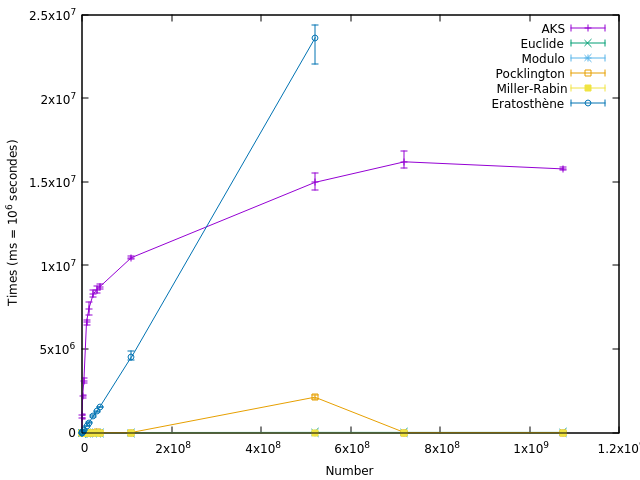
\includegraphics[scale=0.6]{result.png}\end{center}
		\begin{center}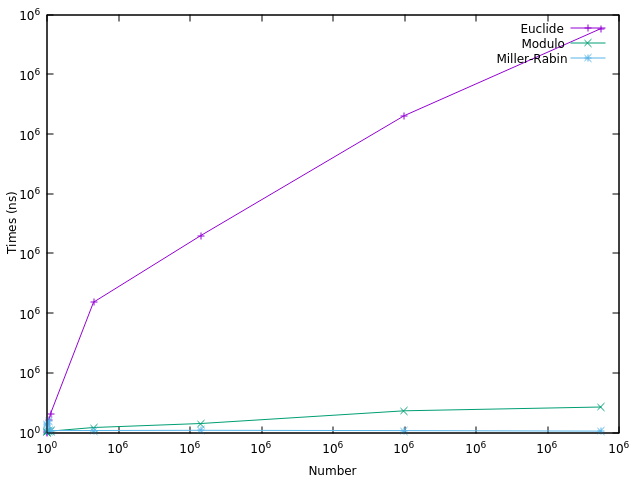
\includegraphics[scale=0.6]{result2.png}\end{center}
	
	Pour commencer nous pouvons observer que les courbes d'évolutions du temps d'exécutions pour les méthodes naïve d'Euclide, d'Eratosthène et de Modulo ont des temps d'exécution très faible pour de petits nombre. Mais les nombres utilisés ici sont de taille raisonnable, mais pour des nombres de l'ordre de $2^{50}$ leur temps d'exécution augmente de façon considérable à cause de leur complexité. Pour l'algorithme de $memory\_bound$ l'utilisation de la mémoire devient beaucoup trop importante à cause du tableau de taile N+1 créer par l'algorithme de crible (Exemple pour 97 on utilise 97 bytes, mais pour $2^{50}$ on aura donc $2^{50}$ bytes utilisé en mémoires). Pour les tests nous nous sommes arreté à $15487253$ car nous sommes limité par les machines que nous avons, notamment la RAM disponible sur celles-ci.\\	
	
	En observant la courbe de Miller Rabin on remarque que le temps d'exécution est très élevé pour les premiers résultats et qu'il accélère grandement pour les derniers, or en regardant les résultats fourni on s'aperçoit que ces derniers sont faux l'algorithme malgré des tests avec un plus grand nombre d'itération renvoie des résultats souvent incorrects lorsque le nombre étudié devient assez grand.\\		
		
		Concernant le test de Pocklington, la courbe ne nous permet pas de définir une évolution précise du temps d'exécution en fonction de la taille du nombre. En effet, la factorisation est la partie théoriquement la plus lourde de cet algorithme, elle est plus ou moins longue en fonction du N en entrée, il est en effet difficile de déduire le temps d’exécution à partir de la taille de N mais le temps d'exécution a quand même tendance a augmenter avec la taille du nombre. Des optimisations de cette partie lourde existe tel que le crible quadratique ou encore le crible algébrique.\\		
		
		En ce qui concerne la courbe pour AKS on peut observer deux ensembles de points qui correspondent a l'étape de détection de la primalité du nombre. En effet, le nombre peut être  détecté comme étant premier à l'étape 4 ou à l'étape 5 de l'algorithme. L'étape 5 est la dernière étape effectué, et celle-ci met un certain temps à se faire, on observe donc cette différence de temps. Passé un certain rang cette différence de temps disparaît ($n > 5690034$)\footnote{https://en.wikipedia.org/wiki/AKS\_primality\_test}).
Sinon la courbe est légèrement croissante, elle va croître doucement compte tenu de la complexité de l’algorithme (O $\log(n)^{12}$).\\

	Pour les deux fonctionnalités sur les nombres hautement composés, l'échantillon suivant : ['2' '120' '240' '360' '720' '840' '1260' '1680' '2520'] a été utilisé pour comparer les deux procédures et observer l'évolution du temps d'exécution.\\
	\begin{center}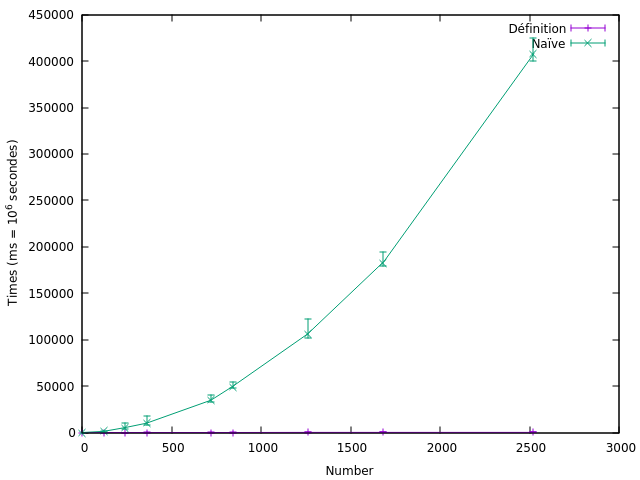
\includegraphics[scale=0.5]{HC.png}\end{center}
	
Nous pouvons observer que la méthode naïve prend énormément de temps pour s'exécuter en comparaison à la méthode appliquant la définition de ce type de nombre. En effet, pour un nombre N donné, la fonction va devoir calculer le nombre de diviseurs pour les N-1 nombres inférieur à N et effectuer N comparaison ce qui engendre beaucoup de latence. Et le temps pour le nombre 2520 est déjà assez élevé  pour un nombre supérieur à $2^{10}$. On peux donc imaginer la courbe accroître plus rapidement pour de très grand nombre. Mais étant limité par notre matériel, nous nous sommes contenté de ce type de nombre.
	\begin{center}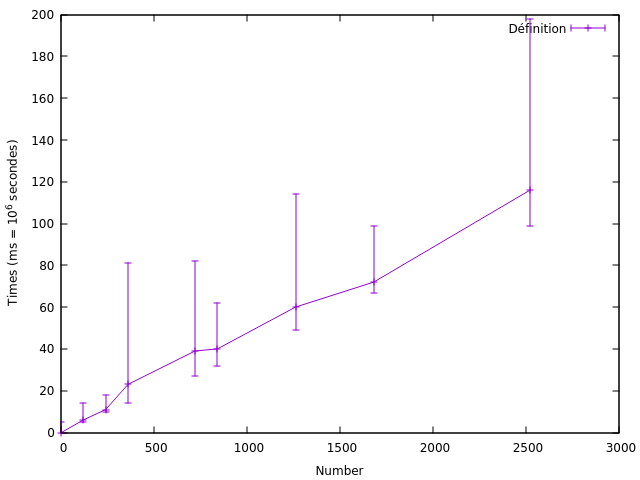
\includegraphics[scale=0.5]{HCdef.png}\end{center}
	 \textit{Zoom sur la courbe pour la méthode appliquant la définition.}
	
	\section{Bilan Technique du Projet}	
		Après l'analyse des résultats nous pouvons constater que les différents tests appliqués possèdent chacun des limites.	
		Tout d'abord, la principale limite du crible d'Eratosthène concerne la taille de son tableau. En effet, pour un nombre N très très grand, le crible va créer un tableau de booléen de taille N+1, ce qui va prendre énormément de place en mémoire, et avec les machines que nous avons à disposition nous sommes très vite limité à cause de la RAM. Puis pour la création de la liste contenant les nombres premiers de 2 jusqu'à N, la fonctionnalité de memory\_bound va devoir parcourir toute les cases du tableau du crible pour remplir sa liste, ce qui engendre une complexité de N pour cette opération de remplissage.\\
		
		La méthode naïve effectue au pire $\sqrt{N}$ divisions euclidiennes. Or cette division euclidienne n'est pas à temps constant. De plus pour un nombre N écrit en base 2, sa longueur vaut $log_2$(N). Notre algorithme effectuera donc $\sqrt{2^{log_2(n)}}$ divisions euclidiennes. Nos méthodes naïves s’exécuteront donc en temps exponentiel. C'est pourquoi ces méthodes très simples et rapides pour de petits nombres deviennent très rapidement non applicable pour de très grand nombres. Le test d'un nombre aux alentour de $2^{64}$ prendra plusieurs années à s’exécuter même sur nos machines actuelles.\\
		
		Ensuite, pour le test de Pocklington la limite principale est le besoin de factoriser le voisin d’en dessous du nombre dont on cherche à valider la primalité, c’est-à-dire N-1 si N est le nombre dont on met la primalité en question. La factorisation des grands nombres est une lourde tâche de calcul de difficulté exponentielle, ainsi même les programmes les plus efficaces demandent énormément de temps, des années voir plus, pour factoriser certaines nombres très grands.
En réalité, nous avons la possibilité de factoriser N-1 qu’en partie, il suffit de factoriser N-1 jusqu’à trouver un A créer à partir des facteurs premiers de N-1 qui respecte les conditions nécessaires pour appliquer le théorème.\\

		Pour Miller-Rabin, les limites concerne le retour de l'algorithme auquel ils nous faut s'assurer que ce dernier ne renvoie pas "premier" pour un nombre composé ou inversement. Pour cela il faut faire plusieurs itérations de l'algorithme, et ce nombre d'itération est difficile à déterminer et si on veut être sûr que le résultat soit correcte le nombre d'itération peut être très élevé ce qui augmente le temps d'exécution nécessaire pour avoir des données correctes.\\	
		
		Concernant l'implémentation de AKS, ce dernier pourrait être sûrement amélioré avec une plus grande connaissance de la bibliothèques NTL utilisé pour l'arithmétique modulaire ou même avec l'utilisation d'autre bibliothèques. De plus une plus grande connaissance en mathématiques aurait permis d'offrir une optimisation pour certaines lignes de code, notamment dans l'étape 5 de l’algorithme. Il aurait aussi été possible d'implémenter une variante de l’algorithme AKS de base qui est plus récente et donc plus optimisé pour un gain de performance certain.
Il est également possible que la bibliothèque NTL fausse les résultats de temps pour l'algorithme AKS. En effet, la bibliothèque effectue certaines vérifications superflues qui ralentiraient le temps d’exécution du test.\\
		
		Enfin, pour les tests d'un nombre hautement composé effectue N calcul du nombre de diviseurs d'un nombre en partant de sa factorisation en nombre premier. C'est pourquoi tout comme les méthodes naïves pour les tests de primalités. Le test en utilisant la méthode naïve d'un nombre aux alentour de $2^{64}$ prendra un temps considérable à s’exécuter même sur nos machines actuelles.
					
	\section{Organisation interne du groupe}
	Pour débuter la programmation de ce projet, il nous fallait en premier lieu établir la répartition du travail de groupe pour que le projet puisse avancer de façon efficace et de manière rapide. Le tableau ci-dessus va ainsi indiquer pour chaque membre du groupe la ou les fonctionnalités pour laquelle il a pu contribuer à l'élaboration: \\
	
	\begin{center}\vspace{-1em}\footnotesize\begin{longtable}{|>{\centering}m{4cm}|>{\centering}m{2cm}|>{\centering}m{2cm}|>{\centering}m{2cm}|>{\centering}m{2cm}|>{\centering\arraybackslash}m{2cm}|}			
		\hline \multicolumn{1}{|c|}{\textbf{Tâches}} & \multicolumn{1}{c|}{\textbf{Jean-Didier}} & \multicolumn{1}{ c|}{\textbf{Maxence}} & \multicolumn{1}{ c|}{\textbf{Romain}} & \multicolumn{1}{ c|}{\textbf{Robin}} & \multicolumn{1}{c|}{\textbf{Damien}}\\
		\hline 	Eratosthène/Memory Bound & x & ~ & ~ & ~ & ~ \\
		\hline 	Euclide/Computation Bound & ~ & x & ~ & ~ & ~ \\
		\hline 	AKS & ~ & ~ & x & ~ & ~ \\
		\hline 	Pocklington & ~ & ~ & ~ & ~ & x \\
		\hline 	Miller-Rabin & ~ & ~ & ~ & x & ~ \\
		\hline 	Highly Composite & x & ~ & ~ & ~ & ~ \\
		\hline 	Cmake  & x & x & ~ & ~ & ~ \\
		\hline  Script & x & x & ~ & ~ & ~ \\
		\hline
	\end{longtable}\vspace{-2.2em}\end{center}	

	\section{Conclusion}
	
	Ce document résume tout ce qui a été établi avant, pendant et après la réalisation de notre projet. Ce projet est donc une application de plusieurs algorithmes pour tester la primalité d'un nombre ou si il est hautement composé. Après une étude des tests sur un échantillon de valeurs on a pu faire plusieurs comparaisons entre ces méthodes. On a pu observer que les méthodes naïves sont très utiles pour les petits nombres mais deviennent très lentes pour les très grands nombres. De plus, Miller-Rabin est un test probabiliste qui pour nous n'est pas très intéressant. En effet ce dernier a une exécution rapide mais une probabilité élevé pour obtenir un résultat non conforme.
		\paragraph{} Dans l'état actuel, on peut revoir avec du recul, la manière avec laquelle notre projet a été réalisé. En effet, nous aurions sûrement revue notre répartition des tâches concernant certains algorithmes comme AKS et Pocklington. Ces derniers ont posés des problèmes pour certains membres du groupe car ces algorithmes ne sont pas faciles à appréhender et demande certaines connaissances notamment en mathématique pour les Polynômes Modulaire pour AKS. Des groupes de 2 pour leur implémentation aurait été préférable.
		\paragraph{} Ce travail a été réalisé par un groupe de 5 personnes. Le sujet, on suppose a été très bien appréhendé par les membre du groupe et l'entente a été excellente. Grâce aux informations préalablement établies lors de notre entretiens avec Monsieur Gougeaud, le travail au sein du groupe a pu être mené de façon assez indépendante, sans générer de conflits ni de problèmes d'organisation.		
		\paragraph{} Pour finir, après observation de nos résultats, nous sommes rentré en phase de réflexion concernant la deuxième étape du projet qui aura lieu pendant le semestre 2. Cette étape consiste à paralléliser l'implémentation faite au cours de ce Semestre. Mais ici tout les tests de primalité ne sont pas forcément parallélisable. Nous pensons actuellement que seul le crible d'Eratosthène est parallélisable et donc il sera de notre ressort de penser à une manière de paralléliser l'implémentation faite ou alors paralléliser les tests fait par le main pour accélérer l'exécution.

\end{document}